\section{The Project}

Lustre was started as a research project in 1999 by Peter Braam, who then
founded \textbf{Cluster File Systems} to continue development on the
project. The first version was released in 2003. Four years later,
\textbf{Sun Microsystems} aquired Cluster File Systems, and in 2010, Sun
itself was bought by the \textbf{Oracle Corporation}.

Oracle was not interested in continuing development or support of the
project, so they discontinued it. Since Lustre is released under the terms
of the GNU General Public License v2, many new organizations could continue
development, including \textbf{Xyratex} and \textbf{Whamcloud} (part of
\textbf{Intel} since 2012).

Several other organizations took over community management and funding of
the project, including \textbf{OpenSFS} (Open Scalable File Systems), whose
slogan is ``keeping Lustre open'', and \textbf{EOFS} (European Open File
Systems), managing community collaboration. Other companies, such as
\textbf{Xyratex}, \textbf{Dell} and \textbf{Terascala}, sell hardware
storage solutions bundled with Lustre software. Braam and other contributors
joined some of these companies and continue working on the project.

Lustre is actively being used in the HPC environment. According to
hcpwire.com, more that 50 percent of the top 50 supercomputers manage their
data using Lustre. This includes the \textbf{Titan}, today's fastest
supercomputer by Cray.

Since Lustre is now being used in huge clusters, the priorities of the project
have changed. While it started out as a science project, for production
environments, the focus had to be shifted to stability instead of features and
performance.

\hspace{2cm}

\begin{figure}[htb]
    \centering
    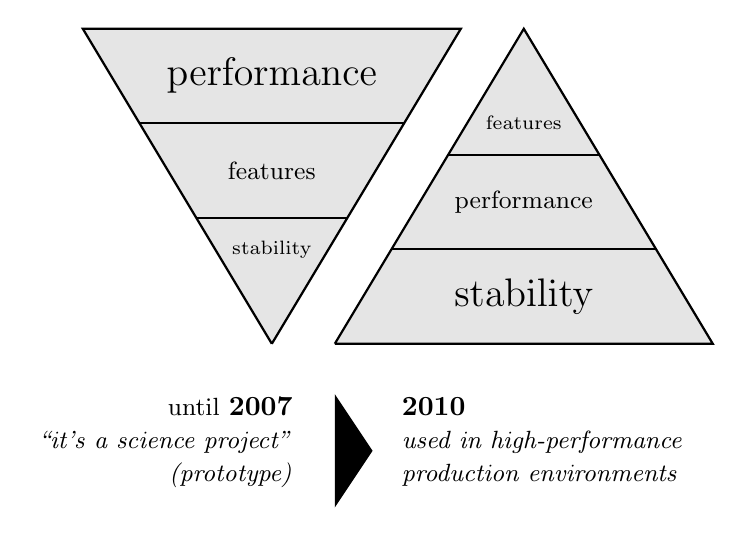
\begin{tikzpicture}[scale=0.8]
        \draw[thick,fill=black!10!white]
            (0, 0) -- (3, 5) -- (-3, 5) -- (0, 0);

        \draw[thick]
            (-2.1, 3.5) -- (2.1, 3.5)
            (-1.2, 2) -- (1.2, 2);

        \node (p1) at (0, 1.5) {\scriptsize stability};
        \node (p2) at (0, 2.75) {\small features};
        \node (p3) at (0, 4.25) {\Large performance};

        \node[align=right,anchor=north] (p7) at (-1.7, -0.7) {{\small{}until} \textbf{2007}\\
            \small\textit{``it's a science project''}\\
            \small\textit{(prototype)}};

        \draw[thick,fill=black!10!white]
            (1, 0) -- (4, 5) -- (7, 0) -- (1, 0);

        \draw[thick]
            (1.9, 1.5) -- (6.1, 1.5)
            (2.8, 3) -- (5.2, 3);

        \node (p6) at (4, 0.75) {\Large stability};
        \node (p5) at (4, 2.25) {\small performance};
        \node (p4) at (4, 3.5) {\scriptsize features};

        \node[align=left,anchor=north] (p8) at (4.3, -0.7) {\textbf{2010}\\
            \small\textit{used in high-performance}\\
            \small\textit{production environments}};

        \fill[fill=black]
            (1.0, -0.8) -- (1.6, -1.7) -- (1.0, -2.6);
    \end{tikzpicture}

    \caption{The change in project priorities}
    \label{fig:priorities}
\end{figure}
